\par \textbf{Introduction}
\newline
\vspace{0.125in}
\par Most Calculus textbooks are long and boring with seemingly endless and sometimes meaningless examples. This text is an attempt to solve that problem with comprehensive yet concise explanations for all of the topics covered in the AP Calculus AB exam for the 2016-17 school year. As the text does not provide many examples, most of the topics are presented in an abstract way and I strongly recommend this text be supplementary to another textbook.\\\par All trigonometry is in radians.\\\par This textbook will have example problems throughout but exercises will be used as more of a checkpoint for the reader rather than homework.\\\par I would also like to thank my first- and second-semester Calculus teacher for teaching me the foundations of Calculus and my third-semester Calculus professor for showing me new ways to use math.\\
\vfill
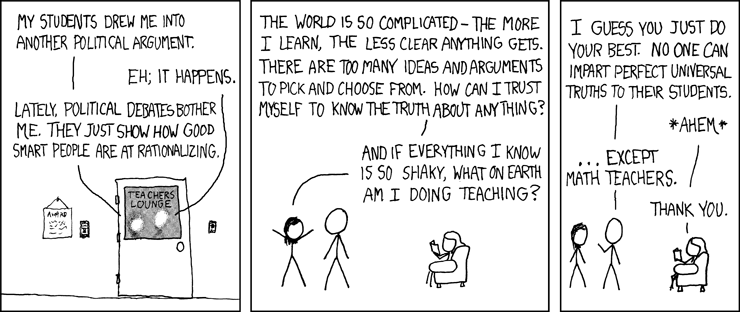
\includegraphics[width=\textwidth]{teachers.png}
\vfill
\par Copyright 2016 by Noah Stockwell
\par Initially published on May 19, 2016
\par Comics used are from xkcd.com, licensed under a Creative Commons Attribution-NonCommercial 2.5 License